\documentclass[twoside]{book}

% Packages required by doxygen
\usepackage{fixltx2e}
\usepackage{calc}
\usepackage{doxygen}
\usepackage[export]{adjustbox} % also loads graphicx
\usepackage{graphicx}
\usepackage[utf8]{inputenc}
\usepackage{makeidx}
\usepackage{multicol}
\usepackage{multirow}
\PassOptionsToPackage{warn}{textcomp}
\usepackage{textcomp}
\usepackage[nointegrals]{wasysym}
\usepackage[table]{xcolor}

% Font selection
\usepackage[T1]{fontenc}
\usepackage[scaled=.90]{helvet}
\usepackage{courier}
\usepackage{amssymb}
\usepackage{sectsty}
\renewcommand{\familydefault}{\sfdefault}
\allsectionsfont{%
  \fontseries{bc}\selectfont%
  \color{darkgray}%
}
\renewcommand{\DoxyLabelFont}{%
  \fontseries{bc}\selectfont%
  \color{darkgray}%
}
\newcommand{\+}{\discretionary{\mbox{\scriptsize$\hookleftarrow$}}{}{}}

% Page & text layout
\usepackage{geometry}
\geometry{%
  a4paper,%
  top=2.5cm,%
  bottom=2.5cm,%
  left=2.5cm,%
  right=2.5cm%
}
\tolerance=750
\hfuzz=15pt
\hbadness=750
\setlength{\emergencystretch}{15pt}
\setlength{\parindent}{0cm}
\setlength{\parskip}{3ex plus 2ex minus 2ex}
\makeatletter
\renewcommand{\paragraph}{%
  \@startsection{paragraph}{4}{0ex}{-1.0ex}{1.0ex}{%
    \normalfont\normalsize\bfseries\SS@parafont%
  }%
}
\renewcommand{\subparagraph}{%
  \@startsection{subparagraph}{5}{0ex}{-1.0ex}{1.0ex}{%
    \normalfont\normalsize\bfseries\SS@subparafont%
  }%
}
\makeatother

% Headers & footers
\usepackage{fancyhdr}
\pagestyle{fancyplain}
\fancyhead[LE]{\fancyplain{}{\bfseries\thepage}}
\fancyhead[CE]{\fancyplain{}{}}
\fancyhead[RE]{\fancyplain{}{\bfseries\leftmark}}
\fancyhead[LO]{\fancyplain{}{\bfseries\rightmark}}
\fancyhead[CO]{\fancyplain{}{}}
\fancyhead[RO]{\fancyplain{}{\bfseries\thepage}}
\fancyfoot[LE]{\fancyplain{}{}}
\fancyfoot[CE]{\fancyplain{}{}}
\fancyfoot[RE]{\fancyplain{}{\bfseries\scriptsize Generated by Doxygen }}
\fancyfoot[LO]{\fancyplain{}{\bfseries\scriptsize Generated by Doxygen }}
\fancyfoot[CO]{\fancyplain{}{}}
\fancyfoot[RO]{\fancyplain{}{}}
\renewcommand{\footrulewidth}{0.4pt}
\renewcommand{\chaptermark}[1]{%
  \markboth{#1}{}%
}
\renewcommand{\sectionmark}[1]{%
  \markright{\thesection\ #1}%
}

% Indices & bibliography
\usepackage{natbib}
\usepackage[titles]{tocloft}
\setcounter{tocdepth}{3}
\setcounter{secnumdepth}{5}
\makeindex

% Hyperlinks (required, but should be loaded last)
\usepackage{ifpdf}
\ifpdf
  \usepackage[pdftex,pagebackref=true]{hyperref}
\else
  \usepackage[ps2pdf,pagebackref=true]{hyperref}
\fi
\hypersetup{%
  colorlinks=true,%
  linkcolor=blue,%
  citecolor=blue,%
  unicode%
}

% Custom commands
\newcommand{\clearemptydoublepage}{%
  \newpage{\pagestyle{empty}\cleardoublepage}%
}

\usepackage{caption}
\captionsetup{labelsep=space,justification=centering,font={bf},singlelinecheck=off,skip=4pt,position=top}

%===== C O N T E N T S =====

\begin{document}

% Titlepage & ToC
\hypersetup{pageanchor=false,
             bookmarksnumbered=true,
             pdfencoding=unicode
            }
\pagenumbering{alph}
\begin{titlepage}
\vspace*{7cm}
\begin{center}%
{\Large My Project }\\
\vspace*{1cm}
{\large Generated by Doxygen 1.8.13}\\
\end{center}
\end{titlepage}
\clearemptydoublepage
\pagenumbering{roman}
\tableofcontents
\clearemptydoublepage
\pagenumbering{arabic}
\hypersetup{pageanchor=true}

%--- Begin generated contents ---
\chapter{Solução Discreta para uma Equação Diferencial Parcial}
\label{index}\hypertarget{index}{}{\bfseries Introdução à Computação Científica C\+I1164} ~\newline
 Trabalho 1 -- Prof. Armando Nicolui ~\newline
 {\bfseries Alunos \+:} ~\newline
 Jackson Rossi Borguezani G\+R\+R20176573 ~\newline
 Roberta Tomigian G\+R\+R20171631\hypertarget{index_introSec}{}\section{Read\+Me}\label{index_introSec}
Dada uma Equação Diferencial Parcial com duas variáveis independentes, discretizamos a malha utilizando Diferenças Finitas Centrais e o método de Gauss-\/\+Seidel para encontrar a possível solução do Sistema Linear.

\begin{DoxyDate}{Date}
03 out 2019 
\end{DoxyDate}

\chapter{P\+DE Solver}
\label{md_README}
\Hypertarget{md_README}
\subsection*{Objetivo}

O objetivo deste trabalho é implementar um programa para calcular a solução discreta para uma Equação Diferencial Parcial com duas variáveis indepententes utilizando Diferenças Finitas centrais de primeira ordem e o método de Gauss-\/\+Seidel. \subsection*{Especificação}

O trabalho consiste em calcular a solução discreta, utilizando Diferenças Finitas Centrais e o Método de Gauss-\/\+Seidel, para a seguinte Equação Diferencial Parcial\+:  onde\+:   O domínio é definido por\+:  Nas fronteiras\+:    

A discretização do domínio deve ser feita em uma malha com espaçamento entre os pontos (0$<$hx,hy$<$pi) calculados a partir do número de pontos em cada dimensão () dados como parâmetro do programa. \begin{DoxyVerb}Escolha uma estrutura de dados eficiente para representar o Sistema Linear resultante;
Escolha um layout eficiente para as variáveis e termos independentes do seu sistema;
Use um vetor nulo como estimativa inicial para a solução;
\end{DoxyVerb}


\subsection*{Execução}

O pacote de software a ser construído deve gerar um executável chamado pde\+Solver, que deve ser invocado da seguinte forma\+: ./pde\+Solver -\/nx $<$nx$>$ -\/ny $<$ny$>$ -\/i $<$max\+Iter$>$ -\/o arquivo\+\_\+saida Onde\+:

-\/nx\+: parâmetro obrigatório definindo o número de pontos a serem calculados na dimensão X. -\/ny\+: parâmetro obrigatório definindo o número de pontos a serem calculados na dimensão Y. -\/i max\+Iter\+: parâmetro obrigatório definindo o número de iterações a serem executadas. -\/o arquivo\+\_\+saida\+: parâmetro no qual arquivo\+\_\+saida é o caminho completo para o arquivo que vai conter a solução (valores da função em cada ponto da grade). Caso este parâmetro não esteja especificado, a saída deve ser stdout Esta solução deve estar formatada para servir de entrada ao comando gnuplot, de forma que ele possa automaticamente gerar o gráfico da função. Além disso, no início do arquivo, deve constar sob a forma de comentários do gnuplot\+: O tempo médio de execução de cada iteração do Método de Gauss-\/\+Seidel O valor do resíduo para cada iteração.

\subparagraph*{}

\section*{Tempo Método GS\+: $<$média de tempo para o cálculo de uma iteração do método, em milisegundos$>$}

\# \section*{Norma L2 do Residuo}

\section*{i=1\+: }

\section*{i=2\+: }

\section*{i=3\+: }

\section*{...}

\subparagraph*{}

\begin{DoxyVerb}Tempo Método GS: deve ser calculado em milisegundos, utilizando-se a função timestamp() especificada aqui. O tempo é calculado a partir do início da iteração do método até a obtenção do vetor solução daquela iteração. O resultado deve ser a média aritmética do tempo de todas iterações.
\end{DoxyVerb}


\subsection*{Makefile}

O arquivo Makefile deve possuir as regras necessárias para compilar os módulos individualmente e gerar o programa executável. As seguintes regras devem existir O\+B\+R\+I\+G\+A\+T\+O\+R\+I\+A\+M\+E\+N\+TE\+: \begin{DoxyVerb}all: compila e produz um executável chamado pdeSolver no diretório login1-login2/;
clean: remove todos os arquivos temporários e os arquivos gerados pelo Makefile (*.o, executável, etc.).
doc: gera a documentação Doxygen em formato html\end{DoxyVerb}
 
\chapter{Class Index}
\section{Class List}
Here are the classes, structs, unions and interfaces with brief descriptions\+:\begin{DoxyCompactList}
\item\contentsline{section}{\hyperlink{structMetrica}{Metrica} \\*Estrutura de dados das métricas usadas na escrita do arquivo }{\pageref{structMetrica}}{}
\item\contentsline{section}{\hyperlink{structSistLinear__t}{Sist\+Linear\+\_\+t} \\*Estrutura de dados do Sistema Linear Pentadiagonal }{\pageref{structSistLinear__t}}{}
\end{DoxyCompactList}

\chapter{File Index}
\section{File List}
Here is a list of all files with brief descriptions\+:\begin{DoxyCompactList}
\item\contentsline{section}{\hyperlink{pdeSolver_8c}{pde\+Solver.\+c} }{\pageref{pdeSolver_8c}}{}
\item\contentsline{section}{\hyperlink{pdeSolver_8h}{pde\+Solver.\+h} }{\pageref{pdeSolver_8h}}{}
\item\contentsline{section}{\hyperlink{SistemasLineares_8c}{Sistemas\+Lineares.\+c} }{\pageref{SistemasLineares_8c}}{}
\item\contentsline{section}{\hyperlink{SistemasLineares_8h}{Sistemas\+Lineares.\+h} }{\pageref{SistemasLineares_8h}}{}
\item\contentsline{section}{\hyperlink{utils_8c}{utils.\+c} }{\pageref{utils_8c}}{}
\item\contentsline{section}{\hyperlink{utils_8h}{utils.\+h} }{\pageref{utils_8h}}{}
\end{DoxyCompactList}

\chapter{Class Documentation}
\hypertarget{structMetrica}{}\section{Metrica Struct Reference}
\label{structMetrica}\index{Metrica@{Metrica}}


Estrutura de dados das métricas usadas na escrita do arquivo.  




{\ttfamily \#include $<$Sistemas\+Lineares.\+h$>$}

\subsection*{Public Attributes}
\begin{DoxyCompactItemize}
\item 
double $\ast$ \hyperlink{structMetrica_a213ed1c24b4afdc96ce9c91f9a6c6301}{norma}
\item 
double \hyperlink{structMetrica_aac2c1968ef74093c6c92364eedfc120e}{media\+Tempo}
\item 
int \hyperlink{structMetrica_a3cdc8f8c5ed005c8f6788d9b33831cc1}{iter}
\end{DoxyCompactItemize}


\subsection{Detailed Description}
Estrutura de dados das métricas usadas na escrita do arquivo. 

\subsection{Member Data Documentation}
\mbox{\Hypertarget{structMetrica_a3cdc8f8c5ed005c8f6788d9b33831cc1}\label{structMetrica_a3cdc8f8c5ed005c8f6788d9b33831cc1}} 
\index{Metrica@{Metrica}!iter@{iter}}
\index{iter@{iter}!Metrica@{Metrica}}
\subsubsection{\texorpdfstring{iter}{iter}}
{\footnotesize\ttfamily int Metrica\+::iter}

Quantidade total de iterações feitas no Gauss-\/\+Seidel \mbox{\Hypertarget{structMetrica_aac2c1968ef74093c6c92364eedfc120e}\label{structMetrica_aac2c1968ef74093c6c92364eedfc120e}} 
\index{Metrica@{Metrica}!media\+Tempo@{media\+Tempo}}
\index{media\+Tempo@{media\+Tempo}!Metrica@{Metrica}}
\subsubsection{\texorpdfstring{media\+Tempo}{mediaTempo}}
{\footnotesize\ttfamily double Metrica\+::media\+Tempo}

Média de tempo de cada iteração do Gauss-\/\+Seidel \mbox{\Hypertarget{structMetrica_a213ed1c24b4afdc96ce9c91f9a6c6301}\label{structMetrica_a213ed1c24b4afdc96ce9c91f9a6c6301}} 
\index{Metrica@{Metrica}!norma@{norma}}
\index{norma@{norma}!Metrica@{Metrica}}
\subsubsection{\texorpdfstring{norma}{norma}}
{\footnotesize\ttfamily double$\ast$ Metrica\+::norma}

Vetor das normas de cada iteração do Gauss-\/\+Seidel 

The documentation for this struct was generated from the following file\+:\begin{DoxyCompactItemize}
\item 
\hyperlink{SistemasLineares_8h}{Sistemas\+Lineares.\+h}\end{DoxyCompactItemize}

\hypertarget{structSistLinear__t}{}\section{Sist\+Linear\+\_\+t Struct Reference}
\label{structSistLinear__t}\index{Sist\+Linear\+\_\+t@{Sist\+Linear\+\_\+t}}


Estrutura de dados do Sistema Linear Pentadiagonal.  




{\ttfamily \#include $<$Sistemas\+Lineares.\+h$>$}

\subsection*{Public Attributes}
\begin{DoxyCompactItemize}
\item 
\hyperlink{SistemasLineares_8h_a0d00e2b3dfadee81331bbb39068570c4}{real\+\_\+t} \hyperlink{structSistLinear__t_ac7f13772865711ff339023fc6ca5ab96}{dp}
\item 
\hyperlink{SistemasLineares_8h_a0d00e2b3dfadee81331bbb39068570c4}{real\+\_\+t} \hyperlink{structSistLinear__t_a2ecc07569471ddd006631f7514960bbb}{ds}
\item 
\hyperlink{SistemasLineares_8h_a0d00e2b3dfadee81331bbb39068570c4}{real\+\_\+t} \hyperlink{structSistLinear__t_a697bd2cd155a3d860f6df76738a5149c}{di}
\item 
\hyperlink{SistemasLineares_8h_a0d00e2b3dfadee81331bbb39068570c4}{real\+\_\+t} \hyperlink{structSistLinear__t_a304278b13b51650f8d6e6482311918c8}{dia}
\item 
\hyperlink{SistemasLineares_8h_a0d00e2b3dfadee81331bbb39068570c4}{real\+\_\+t} \hyperlink{structSistLinear__t_aefdf2d67bee5c6471bae21bb7ced88a6}{dsa}
\item 
\hyperlink{SistemasLineares_8h_a0d00e2b3dfadee81331bbb39068570c4}{real\+\_\+t} $\ast$ \hyperlink{structSistLinear__t_a5f554632eec68e5e0dbea0058c9657ac}{b}
\item 
\hyperlink{SistemasLineares_8h_a0d00e2b3dfadee81331bbb39068570c4}{real\+\_\+t} $\ast$ \hyperlink{structSistLinear__t_a106437fbdef1dee46d7b1c34509e0da1}{x}
\item 
unsigned int \hyperlink{structSistLinear__t_a0f02ce66276316fd835180cf6a033001}{nx}
\item 
unsigned int \hyperlink{structSistLinear__t_a84d8f1f84f050ca4dfc93a4ceaef2b9a}{ny}
\end{DoxyCompactItemize}


\subsection{Detailed Description}
Estrutura de dados do Sistema Linear Pentadiagonal. 

\subsection{Member Data Documentation}
\mbox{\Hypertarget{structSistLinear__t_a5f554632eec68e5e0dbea0058c9657ac}\label{structSistLinear__t_a5f554632eec68e5e0dbea0058c9657ac}} 
\index{Sist\+Linear\+\_\+t@{Sist\+Linear\+\_\+t}!b@{b}}
\index{b@{b}!Sist\+Linear\+\_\+t@{Sist\+Linear\+\_\+t}}
\subsubsection{\texorpdfstring{b}{b}}
{\footnotesize\ttfamily \hyperlink{SistemasLineares_8h_a0d00e2b3dfadee81331bbb39068570c4}{real\+\_\+t}$\ast$ Sist\+Linear\+\_\+t\+::b}

Vetor de termos independentes. \mbox{\Hypertarget{structSistLinear__t_a697bd2cd155a3d860f6df76738a5149c}\label{structSistLinear__t_a697bd2cd155a3d860f6df76738a5149c}} 
\index{Sist\+Linear\+\_\+t@{Sist\+Linear\+\_\+t}!di@{di}}
\index{di@{di}!Sist\+Linear\+\_\+t@{Sist\+Linear\+\_\+t}}
\subsubsection{\texorpdfstring{di}{di}}
{\footnotesize\ttfamily \hyperlink{SistemasLineares_8h_a0d00e2b3dfadee81331bbb39068570c4}{real\+\_\+t} Sist\+Linear\+\_\+t\+::di}

Vetor da diagonal inferior. \mbox{\Hypertarget{structSistLinear__t_a304278b13b51650f8d6e6482311918c8}\label{structSistLinear__t_a304278b13b51650f8d6e6482311918c8}} 
\index{Sist\+Linear\+\_\+t@{Sist\+Linear\+\_\+t}!dia@{dia}}
\index{dia@{dia}!Sist\+Linear\+\_\+t@{Sist\+Linear\+\_\+t}}
\subsubsection{\texorpdfstring{dia}{dia}}
{\footnotesize\ttfamily \hyperlink{SistemasLineares_8h_a0d00e2b3dfadee81331bbb39068570c4}{real\+\_\+t} Sist\+Linear\+\_\+t\+::dia}

Vetor da diagonal inferior afastada. \mbox{\Hypertarget{structSistLinear__t_ac7f13772865711ff339023fc6ca5ab96}\label{structSistLinear__t_ac7f13772865711ff339023fc6ca5ab96}} 
\index{Sist\+Linear\+\_\+t@{Sist\+Linear\+\_\+t}!dp@{dp}}
\index{dp@{dp}!Sist\+Linear\+\_\+t@{Sist\+Linear\+\_\+t}}
\subsubsection{\texorpdfstring{dp}{dp}}
{\footnotesize\ttfamily \hyperlink{SistemasLineares_8h_a0d00e2b3dfadee81331bbb39068570c4}{real\+\_\+t} Sist\+Linear\+\_\+t\+::dp}

Vetor da diagonal principal. \mbox{\Hypertarget{structSistLinear__t_a2ecc07569471ddd006631f7514960bbb}\label{structSistLinear__t_a2ecc07569471ddd006631f7514960bbb}} 
\index{Sist\+Linear\+\_\+t@{Sist\+Linear\+\_\+t}!ds@{ds}}
\index{ds@{ds}!Sist\+Linear\+\_\+t@{Sist\+Linear\+\_\+t}}
\subsubsection{\texorpdfstring{ds}{ds}}
{\footnotesize\ttfamily \hyperlink{SistemasLineares_8h_a0d00e2b3dfadee81331bbb39068570c4}{real\+\_\+t} Sist\+Linear\+\_\+t\+::ds}

Vetor da diagonal superior. \mbox{\Hypertarget{structSistLinear__t_aefdf2d67bee5c6471bae21bb7ced88a6}\label{structSistLinear__t_aefdf2d67bee5c6471bae21bb7ced88a6}} 
\index{Sist\+Linear\+\_\+t@{Sist\+Linear\+\_\+t}!dsa@{dsa}}
\index{dsa@{dsa}!Sist\+Linear\+\_\+t@{Sist\+Linear\+\_\+t}}
\subsubsection{\texorpdfstring{dsa}{dsa}}
{\footnotesize\ttfamily \hyperlink{SistemasLineares_8h_a0d00e2b3dfadee81331bbb39068570c4}{real\+\_\+t} Sist\+Linear\+\_\+t\+::dsa}

Vetor da diagonal superior afastada. \mbox{\Hypertarget{structSistLinear__t_a0f02ce66276316fd835180cf6a033001}\label{structSistLinear__t_a0f02ce66276316fd835180cf6a033001}} 
\index{Sist\+Linear\+\_\+t@{Sist\+Linear\+\_\+t}!nx@{nx}}
\index{nx@{nx}!Sist\+Linear\+\_\+t@{Sist\+Linear\+\_\+t}}
\subsubsection{\texorpdfstring{nx}{nx}}
{\footnotesize\ttfamily unsigned int Sist\+Linear\+\_\+t\+::nx}

Quantidade de pontos em x. \mbox{\Hypertarget{structSistLinear__t_a84d8f1f84f050ca4dfc93a4ceaef2b9a}\label{structSistLinear__t_a84d8f1f84f050ca4dfc93a4ceaef2b9a}} 
\index{Sist\+Linear\+\_\+t@{Sist\+Linear\+\_\+t}!ny@{ny}}
\index{ny@{ny}!Sist\+Linear\+\_\+t@{Sist\+Linear\+\_\+t}}
\subsubsection{\texorpdfstring{ny}{ny}}
{\footnotesize\ttfamily unsigned int Sist\+Linear\+\_\+t\+::ny}

Quantidade de pontos em y. \mbox{\Hypertarget{structSistLinear__t_a106437fbdef1dee46d7b1c34509e0da1}\label{structSistLinear__t_a106437fbdef1dee46d7b1c34509e0da1}} 
\index{Sist\+Linear\+\_\+t@{Sist\+Linear\+\_\+t}!x@{x}}
\index{x@{x}!Sist\+Linear\+\_\+t@{Sist\+Linear\+\_\+t}}
\subsubsection{\texorpdfstring{x}{x}}
{\footnotesize\ttfamily \hyperlink{SistemasLineares_8h_a0d00e2b3dfadee81331bbb39068570c4}{real\+\_\+t}$\ast$ Sist\+Linear\+\_\+t\+::x}

Vetor solução. 

The documentation for this struct was generated from the following file\+:\begin{DoxyCompactItemize}
\item 
\hyperlink{SistemasLineares_8h}{Sistemas\+Lineares.\+h}\end{DoxyCompactItemize}

\chapter{File Documentation}
\hypertarget{pdeSolver_8c}{}\section{pde\+Solver.\+c File Reference}
\label{pdeSolver_8c}\index{pde\+Solver.\+c@{pde\+Solver.\+c}}
{\ttfamily \#include $<$stdio.\+h$>$}\\*
{\ttfamily \#include $<$stdlib.\+h$>$}\\*
{\ttfamily \#include $<$string.\+h$>$}\\*
{\ttfamily \#include $<$time.\+h$>$}\\*
{\ttfamily \#include $<$sys/time.\+h$>$}\\*
{\ttfamily \#include $<$math.\+h$>$}\\*
{\ttfamily \#include \char`\"{}utils.\+h\char`\"{}}\\*
{\ttfamily \#include \char`\"{}Sistemas\+Lineares.\+h\char`\"{}}\\*
{\ttfamily \#include \char`\"{}pde\+Solver.\+h\char`\"{}}\\*
{\ttfamily \#include $<$getopt.\+h$>$}\\*
Include dependency graph for pde\+Solver.\+c\+:

\hypertarget{pdeSolver_8h}{}\section{pde\+Solver.\+h File Reference}
\label{pdeSolver_8h}\index{pde\+Solver.\+h@{pde\+Solver.\+h}}
This graph shows which files directly or indirectly include this file\+:
% FIG 0
\subsection*{Functions}
\begin{DoxyCompactItemize}
\item 
void \hyperlink{pdeSolver_8h_a1c0f6eee3572973fe263b0125a72b889}{gera\+\_\+matriz} (\hyperlink{structSistLinear__t}{Sist\+Linear\+\_\+t} $\ast$SL)
\begin{DoxyCompactList}\small\item\em Monta a matriz pentadiagonal do SL. \end{DoxyCompactList}\item 
void \hyperlink{pdeSolver_8h_a4959ff3519b19f59fb4fc2c62e658d30}{gera\+\_\+vetor\+\_\+b} (\hyperlink{structSistLinear__t}{Sist\+Linear\+\_\+t} $\ast$SL)
\begin{DoxyCompactList}\small\item\em Calcula o vetor dos termos independentes B do SL. \end{DoxyCompactList}\end{DoxyCompactItemize}


\subsection{Function Documentation}
\index{pde\+Solver.\+h@{pde\+Solver.\+h}!gera\+\_\+matriz@{gera\+\_\+matriz}}
\index{gera\+\_\+matriz@{gera\+\_\+matriz}!pde\+Solver.\+h@{pde\+Solver.\+h}}
\subsubsection[{\texorpdfstring{gera\+\_\+matriz(\+Sist\+Linear\+\_\+t $\ast$\+S\+L)}{gera_matriz(SistLinear_t *SL)}}]{\setlength{\rightskip}{0pt plus 5cm}void gera\+\_\+matriz (
\begin{DoxyParamCaption}
\item[{{\bf Sist\+Linear\+\_\+t} $\ast$}]{SL}
\end{DoxyParamCaption}
)}\hypertarget{pdeSolver_8h_a1c0f6eee3572973fe263b0125a72b889}{}\label{pdeSolver_8h_a1c0f6eee3572973fe263b0125a72b889}


Monta a matriz pentadiagonal do SL. 

Função que gera a matriz de coeficientes A.


\begin{DoxyParams}{Parameters}
{\em SL} & Ponteiro do Sistema Linear\\
\hline
\end{DoxyParams}
A função libera todos os ponteiros da estrutura do Sistema Linear.


\begin{DoxyParams}{Parameters}
{\em SL} & é o Sistema Linear\\
\hline
\end{DoxyParams}
Essa função gera a matriz de coeficientes a partir da aproximação de valores da Equação Diferencial Parcial \index{pde\+Solver.\+h@{pde\+Solver.\+h}!gera\+\_\+vetor\+\_\+b@{gera\+\_\+vetor\+\_\+b}}
\index{gera\+\_\+vetor\+\_\+b@{gera\+\_\+vetor\+\_\+b}!pde\+Solver.\+h@{pde\+Solver.\+h}}
\subsubsection[{\texorpdfstring{gera\+\_\+vetor\+\_\+b(\+Sist\+Linear\+\_\+t $\ast$\+S\+L)}{gera_vetor_b(SistLinear_t *SL)}}]{\setlength{\rightskip}{0pt plus 5cm}void gera\+\_\+vetor\+\_\+b (
\begin{DoxyParamCaption}
\item[{{\bf Sist\+Linear\+\_\+t} $\ast$}]{SL}
\end{DoxyParamCaption}
)}\hypertarget{pdeSolver_8h_a4959ff3519b19f59fb4fc2c62e658d30}{}\label{pdeSolver_8h_a4959ff3519b19f59fb4fc2c62e658d30}


Calcula o vetor dos termos independentes B do SL. 

Função que gera o vetor de termos independentes b.


\begin{DoxyParams}{Parameters}
{\em SL} & Ponteiro do Sistema Linear\\
\hline
\end{DoxyParams}
A função libera todos os ponteiros da estrutura do Sistema Linear.


\begin{DoxyParams}{Parameters}
{\em SL} & é o Sistema Linear\\
\hline
\end{DoxyParams}
Essa função gera o vetor de termos independentes b a partir da aproximação de valores da Equação Diferencial Parcial 
\hypertarget{README_8md}{}\section{R\+E\+A\+D\+M\+E.\+md File Reference}
\label{README_8md}\index{R\+E\+A\+D\+M\+E.\+md@{R\+E\+A\+D\+M\+E.\+md}}

\hypertarget{SistemasLineares_8c}{}\section{Sistemas\+Lineares.\+c File Reference}
\label{SistemasLineares_8c}\index{Sistemas\+Lineares.\+c@{Sistemas\+Lineares.\+c}}
{\ttfamily \#include $<$stdio.\+h$>$}\newline
{\ttfamily \#include $<$math.\+h$>$}\newline
{\ttfamily \#include $<$stdlib.\+h$>$}\newline
{\ttfamily \#include \char`\"{}Sistemas\+Lineares.\+h\char`\"{}}\newline
{\ttfamily \#include \char`\"{}utils.\+h\char`\"{}}\newline
Include dependency graph for Sistemas\+Lineares.\+c\+:
\nopagebreak
\begin{figure}[H]
\begin{center}
\leavevmode
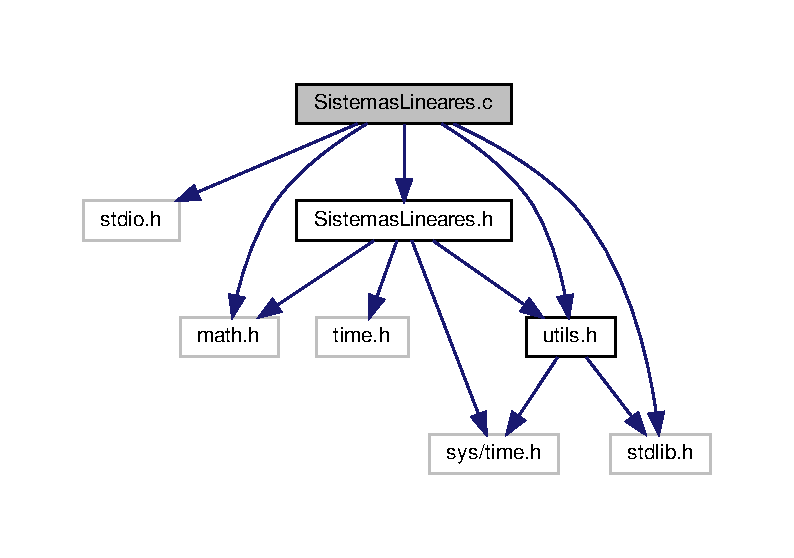
\includegraphics[width=350pt]{SistemasLineares_8c__incl}
\end{center}
\end{figure}
\subsection*{Functions}
\begin{DoxyCompactItemize}
\item 
\hyperlink{structSistLinear__t}{Sist\+Linear\+\_\+t} $\ast$ \hyperlink{SistemasLineares_8c_ad84846c03b1d7cdb3e86725335a8d57d}{aloca\+Sist\+Linear} (unsigned int nx, unsigned int ny)
\begin{DoxyCompactList}\small\item\em Alocação do Sistema Linear Pentadiagonal. \end{DoxyCompactList}\item 
\hyperlink{structMetrica}{Metrica} $\ast$ \hyperlink{SistemasLineares_8c_a0fa56411c2db5133e91703b6d8ff3b5c}{aloca\+Metrica} (unsigned int nx, unsigned int ny, int max\+Iter)
\begin{DoxyCompactList}\small\item\em Aloca e inicia a estrutura de dados métrica. \end{DoxyCompactList}\item 
void \hyperlink{SistemasLineares_8c_a4c76f8fde8fb7cf7848927226cfdab01}{inicializa\+Sist\+Linear} (\hyperlink{structSistLinear__t}{Sist\+Linear\+\_\+t} $\ast$SL, int x, int y)
\begin{DoxyCompactList}\small\item\em Inicialização do Sistema Linear com zeros. \end{DoxyCompactList}\item 
void \hyperlink{SistemasLineares_8c_ae7acbfa45287b31c524467ab6d3f77e3}{libera\+Sist\+Linear} (\hyperlink{structSistLinear__t}{Sist\+Linear\+\_\+t} $\ast$SL)
\begin{DoxyCompactList}\small\item\em Liberação dos Ponteiros do Sistema Linear. \end{DoxyCompactList}\item 
int \hyperlink{SistemasLineares_8c_a53fd7846d6ddc652216c50d032ae7f8c}{gauss\+Seidel} (\hyperlink{structSistLinear__t}{Sist\+Linear\+\_\+t} $\ast$SL, int max\+Iter, \hyperlink{structMetrica}{Metrica} $\ast$P)
\item 
double \hyperlink{SistemasLineares_8c_a7b3b187094b9ddbf49c4bed5e5f1cda2}{norma\+L2\+Residuo} (\hyperlink{structSistLinear__t}{Sist\+Linear\+\_\+t} $\ast$SL)
\begin{DoxyCompactList}\small\item\em Cálculo da Norma\+L2. \end{DoxyCompactList}\end{DoxyCompactItemize}


\subsection{Detailed Description}
\begin{DoxyAuthor}{Author}
Jackson Borguezani \& Roberta Tomigian 
\end{DoxyAuthor}


\subsection{Function Documentation}
\mbox{\Hypertarget{SistemasLineares_8c_a0fa56411c2db5133e91703b6d8ff3b5c}\label{SistemasLineares_8c_a0fa56411c2db5133e91703b6d8ff3b5c}} 
\index{Sistemas\+Lineares.\+c@{Sistemas\+Lineares.\+c}!aloca\+Metrica@{aloca\+Metrica}}
\index{aloca\+Metrica@{aloca\+Metrica}!Sistemas\+Lineares.\+c@{Sistemas\+Lineares.\+c}}
\subsubsection{\texorpdfstring{aloca\+Metrica()}{alocaMetrica()}}
{\footnotesize\ttfamily \hyperlink{structMetrica}{Metrica} $\ast$ aloca\+Metrica (\begin{DoxyParamCaption}\item[{unsigned int}]{nx,  }\item[{unsigned int}]{ny,  }\item[{int}]{max\+Iter }\end{DoxyParamCaption})}



Aloca e inicia a estrutura de dados métrica. 


\begin{DoxyParams}{Parameters}
{\em nx} & Número de pontos a serem calculados no eixo x\\
\hline
{\em ny} & Número de pontos a serem calculados no eixo y\\
\hline
{\em max\+Iter} & Número máximo de iterações \\
\hline
\end{DoxyParams}
\mbox{\Hypertarget{SistemasLineares_8c_ad84846c03b1d7cdb3e86725335a8d57d}\label{SistemasLineares_8c_ad84846c03b1d7cdb3e86725335a8d57d}} 
\index{Sistemas\+Lineares.\+c@{Sistemas\+Lineares.\+c}!aloca\+Sist\+Linear@{aloca\+Sist\+Linear}}
\index{aloca\+Sist\+Linear@{aloca\+Sist\+Linear}!Sistemas\+Lineares.\+c@{Sistemas\+Lineares.\+c}}
\subsubsection{\texorpdfstring{aloca\+Sist\+Linear()}{alocaSistLinear()}}
{\footnotesize\ttfamily \hyperlink{structSistLinear__t}{Sist\+Linear\+\_\+t} $\ast$ aloca\+Sist\+Linear (\begin{DoxyParamCaption}\item[{unsigned int}]{nx,  }\item[{unsigned int}]{ny }\end{DoxyParamCaption})}



Alocação do Sistema Linear Pentadiagonal. 


\begin{DoxyParams}{Parameters}
{\em nx} & Número de pontos a serem calculados no eixo x\\
\hline
{\em ny} & Número de pontos a serem calculados no eixo y\\
\hline
\end{DoxyParams}
Função responsável por alocar dinamicamente os vetores do SL. \mbox{\Hypertarget{SistemasLineares_8c_a53fd7846d6ddc652216c50d032ae7f8c}\label{SistemasLineares_8c_a53fd7846d6ddc652216c50d032ae7f8c}} 
\index{Sistemas\+Lineares.\+c@{Sistemas\+Lineares.\+c}!gauss\+Seidel@{gauss\+Seidel}}
\index{gauss\+Seidel@{gauss\+Seidel}!Sistemas\+Lineares.\+c@{Sistemas\+Lineares.\+c}}
\subsubsection{\texorpdfstring{gauss\+Seidel()}{gaussSeidel()}}
{\footnotesize\ttfamily int gauss\+Seidel (\begin{DoxyParamCaption}\item[{\hyperlink{structSistLinear__t}{Sist\+Linear\+\_\+t} $\ast$}]{SL,  }\item[{int}]{max\+Iter,  }\item[{\hyperlink{structMetrica}{Metrica} $\ast$}]{P }\end{DoxyParamCaption})}

\mbox{\Hypertarget{SistemasLineares_8c_a4c76f8fde8fb7cf7848927226cfdab01}\label{SistemasLineares_8c_a4c76f8fde8fb7cf7848927226cfdab01}} 
\index{Sistemas\+Lineares.\+c@{Sistemas\+Lineares.\+c}!inicializa\+Sist\+Linear@{inicializa\+Sist\+Linear}}
\index{inicializa\+Sist\+Linear@{inicializa\+Sist\+Linear}!Sistemas\+Lineares.\+c@{Sistemas\+Lineares.\+c}}
\subsubsection{\texorpdfstring{inicializa\+Sist\+Linear()}{inicializaSistLinear()}}
{\footnotesize\ttfamily void inicializa\+Sist\+Linear (\begin{DoxyParamCaption}\item[{\hyperlink{structSistLinear__t}{Sist\+Linear\+\_\+t} $\ast$}]{SL,  }\item[{int}]{x,  }\item[{int}]{y }\end{DoxyParamCaption})}



Inicialização do Sistema Linear com zeros. 


\begin{DoxyParams}{Parameters}
{\em SL} & Ponteiro do Sistema Linear\\
\hline
{\em x} & Número de pontos a serem calculados no eixo x\\
\hline
{\em y} & Número de pontos a serem calculados no eixo y \\
\hline
\end{DoxyParams}
\mbox{\Hypertarget{SistemasLineares_8c_ae7acbfa45287b31c524467ab6d3f77e3}\label{SistemasLineares_8c_ae7acbfa45287b31c524467ab6d3f77e3}} 
\index{Sistemas\+Lineares.\+c@{Sistemas\+Lineares.\+c}!libera\+Sist\+Linear@{libera\+Sist\+Linear}}
\index{libera\+Sist\+Linear@{libera\+Sist\+Linear}!Sistemas\+Lineares.\+c@{Sistemas\+Lineares.\+c}}
\subsubsection{\texorpdfstring{libera\+Sist\+Linear()}{liberaSistLinear()}}
{\footnotesize\ttfamily void libera\+Sist\+Linear (\begin{DoxyParamCaption}\item[{\hyperlink{structSistLinear__t}{Sist\+Linear\+\_\+t} $\ast$}]{SL }\end{DoxyParamCaption})}



Liberação dos Ponteiros do Sistema Linear. 


\begin{DoxyParams}{Parameters}
{\em SL} & Ponteiro do Sistema Linear\\
\hline
\end{DoxyParams}
A função libera todos os ponteiros da estrutura do Sistema Linear. \mbox{\Hypertarget{SistemasLineares_8c_a7b3b187094b9ddbf49c4bed5e5f1cda2}\label{SistemasLineares_8c_a7b3b187094b9ddbf49c4bed5e5f1cda2}} 
\index{Sistemas\+Lineares.\+c@{Sistemas\+Lineares.\+c}!norma\+L2\+Residuo@{norma\+L2\+Residuo}}
\index{norma\+L2\+Residuo@{norma\+L2\+Residuo}!Sistemas\+Lineares.\+c@{Sistemas\+Lineares.\+c}}
\subsubsection{\texorpdfstring{norma\+L2\+Residuo()}{normaL2Residuo()}}
{\footnotesize\ttfamily double norma\+L2\+Residuo (\begin{DoxyParamCaption}\item[{\hyperlink{structSistLinear__t}{Sist\+Linear\+\_\+t} $\ast$}]{SL }\end{DoxyParamCaption})}



Cálculo da Norma\+L2. 


\begin{DoxyParams}{Parameters}
{\em SL} & Ponteiro do Sistema Linear \\
\hline
\end{DoxyParams}

\hypertarget{SistemasLineares_8h}{}\section{Sistemas\+Lineares.\+h File Reference}
\label{SistemasLineares_8h}\index{Sistemas\+Lineares.\+h@{Sistemas\+Lineares.\+h}}
{\ttfamily \#include $<$time.\+h$>$}\\*
{\ttfamily \#include $<$sys/time.\+h$>$}\\*
{\ttfamily \#include $<$math.\+h$>$}\\*
{\ttfamily \#include \char`\"{}utils.\+h\char`\"{}}\\*
Include dependency graph for Sistemas\+Lineares.\+h\+:
% FIG 0
This graph shows which files directly or indirectly include this file\+:
% FIG 1
\subsection*{Classes}
\begin{DoxyCompactItemize}
\item 
struct \hyperlink{structSistLinear__t}{Sist\+Linear\+\_\+t}
\begin{DoxyCompactList}\small\item\em Estrutura de dados do Sistema Linear Pentadiagonal. \end{DoxyCompactList}\end{DoxyCompactItemize}
\subsection*{Macros}
\begin{DoxyCompactItemize}
\item 
\#define \hyperlink{SistemasLineares_8h_a6ebf6899d6c1c8b7b9d09be872c05aae}{E\+PS}~1.\+0e-\/4
\end{DoxyCompactItemize}
\subsection*{Typedefs}
\begin{DoxyCompactItemize}
\item 
typedef double \hyperlink{SistemasLineares_8h_a0d00e2b3dfadee81331bbb39068570c4}{real\+\_\+t}
\end{DoxyCompactItemize}
\subsection*{Functions}
\begin{DoxyCompactItemize}
\item 
\hyperlink{structSistLinear__t}{Sist\+Linear\+\_\+t} $\ast$ \hyperlink{SistemasLineares_8h_acdbd7298023b1063f141df043ed78f2f}{aloca\+Sist\+Linear} (unsigned int nx, unsigned int ny)
\begin{DoxyCompactList}\small\item\em Alocação do Sistema Linear Pentadiagonal. \end{DoxyCompactList}\item 
void \hyperlink{SistemasLineares_8h_a4c76f8fde8fb7cf7848927226cfdab01}{inicializa\+Sist\+Linear} (\hyperlink{structSistLinear__t}{Sist\+Linear\+\_\+t} $\ast$SL, int x, int y)
\begin{DoxyCompactList}\small\item\em Inicialização do Sistema Linear com zeros. \end{DoxyCompactList}\item 
void \hyperlink{SistemasLineares_8h_ae7acbfa45287b31c524467ab6d3f77e3}{libera\+Sist\+Linear} (\hyperlink{structSistLinear__t}{Sist\+Linear\+\_\+t} $\ast$SL)
\begin{DoxyCompactList}\small\item\em Liberação dos Ponteiros do Sistema Linear. \end{DoxyCompactList}\item 
int \hyperlink{SistemasLineares_8h_aa8b9986acaa8f53f82eac42362fde8c1}{gauss\+Seidel} (\hyperlink{structSistLinear__t}{Sist\+Linear\+\_\+t} $\ast$SL, int max\+Iter)
\begin{DoxyCompactList}\small\item\em Método da Gauss-\/\+Seidel. \end{DoxyCompactList}\item 
double \hyperlink{SistemasLineares_8h_a7b3b187094b9ddbf49c4bed5e5f1cda2}{norma\+L2\+Residuo} (\hyperlink{structSistLinear__t}{Sist\+Linear\+\_\+t} $\ast$SL)
\begin{DoxyCompactList}\small\item\em Cálculo da Norma\+L2. \end{DoxyCompactList}\end{DoxyCompactItemize}


\subsection{Detailed Description}
\begin{DoxyAuthor}{Author}
Jackson Borguezani \& Roberta Tomigian 
\end{DoxyAuthor}


\subsection{Macro Definition Documentation}
\index{Sistemas\+Lineares.\+h@{Sistemas\+Lineares.\+h}!E\+PS@{E\+PS}}
\index{E\+PS@{E\+PS}!Sistemas\+Lineares.\+h@{Sistemas\+Lineares.\+h}}
\subsubsection[{\texorpdfstring{E\+PS}{EPS}}]{\setlength{\rightskip}{0pt plus 5cm}\#define E\+PS~1.\+0e-\/4}\hypertarget{SistemasLineares_8h_a6ebf6899d6c1c8b7b9d09be872c05aae}{}\label{SistemasLineares_8h_a6ebf6899d6c1c8b7b9d09be872c05aae}


\subsection{Typedef Documentation}
\index{Sistemas\+Lineares.\+h@{Sistemas\+Lineares.\+h}!real\+\_\+t@{real\+\_\+t}}
\index{real\+\_\+t@{real\+\_\+t}!Sistemas\+Lineares.\+h@{Sistemas\+Lineares.\+h}}
\subsubsection[{\texorpdfstring{real\+\_\+t}{real_t}}]{\setlength{\rightskip}{0pt plus 5cm}typedef double {\bf real\+\_\+t}}\hypertarget{SistemasLineares_8h_a0d00e2b3dfadee81331bbb39068570c4}{}\label{SistemasLineares_8h_a0d00e2b3dfadee81331bbb39068570c4}


\subsection{Function Documentation}
\index{Sistemas\+Lineares.\+h@{Sistemas\+Lineares.\+h}!aloca\+Sist\+Linear@{aloca\+Sist\+Linear}}
\index{aloca\+Sist\+Linear@{aloca\+Sist\+Linear}!Sistemas\+Lineares.\+h@{Sistemas\+Lineares.\+h}}
\subsubsection[{\texorpdfstring{aloca\+Sist\+Linear(unsigned int nx, unsigned int ny)}{alocaSistLinear(unsigned int nx, unsigned int ny)}}]{\setlength{\rightskip}{0pt plus 5cm}{\bf Sist\+Linear\+\_\+t}$\ast$ aloca\+Sist\+Linear (
\begin{DoxyParamCaption}
\item[{unsigned int}]{nx, }
\item[{unsigned int}]{ny}
\end{DoxyParamCaption}
)}\hypertarget{SistemasLineares_8h_acdbd7298023b1063f141df043ed78f2f}{}\label{SistemasLineares_8h_acdbd7298023b1063f141df043ed78f2f}


Alocação do Sistema Linear Pentadiagonal. 


\begin{DoxyParams}{Parameters}
{\em nx} & Número de pontos a serem calculados no eixo x\\
\hline
{\em ny} & Número de pontos a serem calculados no eixo y\\
\hline
\end{DoxyParams}
Função responsável por alocar dinamicamente os vetores do SL. \index{Sistemas\+Lineares.\+h@{Sistemas\+Lineares.\+h}!gauss\+Seidel@{gauss\+Seidel}}
\index{gauss\+Seidel@{gauss\+Seidel}!Sistemas\+Lineares.\+h@{Sistemas\+Lineares.\+h}}
\subsubsection[{\texorpdfstring{gauss\+Seidel(\+Sist\+Linear\+\_\+t $\ast$\+S\+L, int max\+Iter)}{gaussSeidel(SistLinear_t *SL, int maxIter)}}]{\setlength{\rightskip}{0pt plus 5cm}int gauss\+Seidel (
\begin{DoxyParamCaption}
\item[{{\bf Sist\+Linear\+\_\+t} $\ast$}]{SL, }
\item[{int}]{max\+Iter}
\end{DoxyParamCaption}
)}\hypertarget{SistemasLineares_8h_aa8b9986acaa8f53f82eac42362fde8c1}{}\label{SistemasLineares_8h_aa8b9986acaa8f53f82eac42362fde8c1}


Método da Gauss-\/\+Seidel. 


\begin{DoxyParams}{Parameters}
{\em SL} & Ponteiro do Sistema Linear\\
\hline
{\em max\+Iter} & Número máximo de iterações\\
\hline
\end{DoxyParams}
Esta função calcula a solução de um sistema linear pentadiagonal, com estrutura de dados em vetores.

Erros possíveis no metodo de Gauss-\/\+Seidel

· Erro (-\/1) D\+I\+V\+I\+S\+A\+O\+\_\+\+P\+O\+R\+\_\+0\+: Caso a diagonal principal seja zero, não é possível calcular a solução pois teremos uma divisao por 0

· Erro (-\/2) A\+T\+I\+N\+G\+I\+U\+\_\+\+M\+A\+X\+\_\+\+I\+T\+E\+R\+A\+C\+O\+ES\+: Ocorre quando o número máximo de iterações, passado por parâmetro, é atingido \index{Sistemas\+Lineares.\+h@{Sistemas\+Lineares.\+h}!inicializa\+Sist\+Linear@{inicializa\+Sist\+Linear}}
\index{inicializa\+Sist\+Linear@{inicializa\+Sist\+Linear}!Sistemas\+Lineares.\+h@{Sistemas\+Lineares.\+h}}
\subsubsection[{\texorpdfstring{inicializa\+Sist\+Linear(\+Sist\+Linear\+\_\+t $\ast$\+S\+L, int x, int y)}{inicializaSistLinear(SistLinear_t *SL, int x, int y)}}]{\setlength{\rightskip}{0pt plus 5cm}void inicializa\+Sist\+Linear (
\begin{DoxyParamCaption}
\item[{{\bf Sist\+Linear\+\_\+t} $\ast$}]{SL, }
\item[{int}]{x, }
\item[{int}]{y}
\end{DoxyParamCaption}
)}\hypertarget{SistemasLineares_8h_a4c76f8fde8fb7cf7848927226cfdab01}{}\label{SistemasLineares_8h_a4c76f8fde8fb7cf7848927226cfdab01}


Inicialização do Sistema Linear com zeros. 


\begin{DoxyParams}{Parameters}
{\em SL} & Ponteiro do Sistema Linear\\
\hline
{\em x} & Número de pontos a serem calculados no eixo x\\
\hline
{\em y} & Número de pontos a serem calculados no eixo y \\
\hline
\end{DoxyParams}
\index{Sistemas\+Lineares.\+h@{Sistemas\+Lineares.\+h}!libera\+Sist\+Linear@{libera\+Sist\+Linear}}
\index{libera\+Sist\+Linear@{libera\+Sist\+Linear}!Sistemas\+Lineares.\+h@{Sistemas\+Lineares.\+h}}
\subsubsection[{\texorpdfstring{libera\+Sist\+Linear(\+Sist\+Linear\+\_\+t $\ast$\+S\+L)}{liberaSistLinear(SistLinear_t *SL)}}]{\setlength{\rightskip}{0pt plus 5cm}void libera\+Sist\+Linear (
\begin{DoxyParamCaption}
\item[{{\bf Sist\+Linear\+\_\+t} $\ast$}]{SL}
\end{DoxyParamCaption}
)}\hypertarget{SistemasLineares_8h_ae7acbfa45287b31c524467ab6d3f77e3}{}\label{SistemasLineares_8h_ae7acbfa45287b31c524467ab6d3f77e3}


Liberação dos Ponteiros do Sistema Linear. 


\begin{DoxyParams}{Parameters}
{\em SL} & Ponteiro do Sistema Linear\\
\hline
\end{DoxyParams}
A função libera todos os ponteiros da estrutura do Sistema Linear. \index{Sistemas\+Lineares.\+h@{Sistemas\+Lineares.\+h}!norma\+L2\+Residuo@{norma\+L2\+Residuo}}
\index{norma\+L2\+Residuo@{norma\+L2\+Residuo}!Sistemas\+Lineares.\+h@{Sistemas\+Lineares.\+h}}
\subsubsection[{\texorpdfstring{norma\+L2\+Residuo(\+Sist\+Linear\+\_\+t $\ast$\+S\+L)}{normaL2Residuo(SistLinear_t *SL)}}]{\setlength{\rightskip}{0pt plus 5cm}double norma\+L2\+Residuo (
\begin{DoxyParamCaption}
\item[{{\bf Sist\+Linear\+\_\+t} $\ast$}]{SL}
\end{DoxyParamCaption}
)}\hypertarget{SistemasLineares_8h_a7b3b187094b9ddbf49c4bed5e5f1cda2}{}\label{SistemasLineares_8h_a7b3b187094b9ddbf49c4bed5e5f1cda2}


Cálculo da Norma\+L2. 


\begin{DoxyParams}{Parameters}
{\em SL} & Ponteiro do Sistema Linear \\
\hline
\end{DoxyParams}

\hypertarget{utils_8c}{}\section{utils.\+c File Reference}
\label{utils_8c}\index{utils.\+c@{utils.\+c}}
{\ttfamily \#include \char`\"{}utils.\+h\char`\"{}}\newline
Include dependency graph for utils.\+c\+:
\nopagebreak
\begin{figure}[H]
\begin{center}
\leavevmode
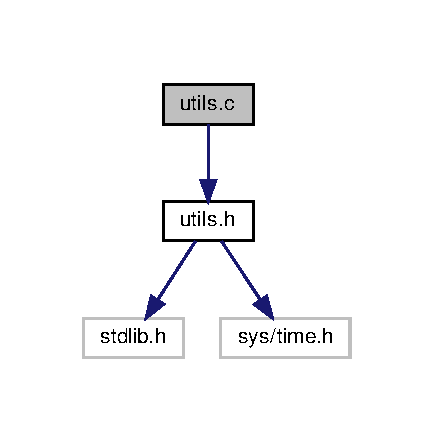
\includegraphics[width=208pt]{utils_8c__incl}
\end{center}
\end{figure}
\subsection*{Functions}
\begin{DoxyCompactItemize}
\item 
double \hyperlink{utils_8c_ad1f75d4b6d05731f71dd8fe6ee54bfeb}{timestamp} (void)
\end{DoxyCompactItemize}


\subsection{Function Documentation}
\mbox{\Hypertarget{utils_8c_ad1f75d4b6d05731f71dd8fe6ee54bfeb}\label{utils_8c_ad1f75d4b6d05731f71dd8fe6ee54bfeb}} 
\index{utils.\+c@{utils.\+c}!timestamp@{timestamp}}
\index{timestamp@{timestamp}!utils.\+c@{utils.\+c}}
\subsubsection{\texorpdfstring{timestamp()}{timestamp()}}
{\footnotesize\ttfamily double timestamp (\begin{DoxyParamCaption}\item[{void}]{ }\end{DoxyParamCaption})}


\hypertarget{utils_8h}{}\section{utils.\+h File Reference}
\label{utils_8h}\index{utils.\+h@{utils.\+h}}
{\ttfamily \#include $<$stdlib.\+h$>$}\newline
{\ttfamily \#include $<$sys/time.\+h$>$}\newline
Include dependency graph for utils.\+h\+:
\nopagebreak
\begin{figure}[H]
\begin{center}
\leavevmode
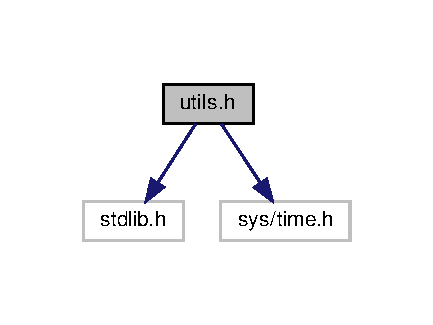
\includegraphics[width=208pt]{utils_8h__incl}
\end{center}
\end{figure}
This graph shows which files directly or indirectly include this file\+:
\nopagebreak
\begin{figure}[H]
\begin{center}
\leavevmode
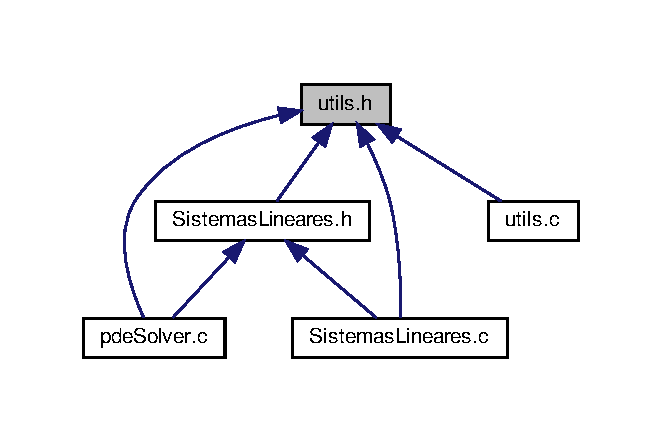
\includegraphics[width=318pt]{utils_8h__dep__incl}
\end{center}
\end{figure}
\subsection*{Functions}
\begin{DoxyCompactItemize}
\item 
double \hyperlink{utils_8h_ad1f75d4b6d05731f71dd8fe6ee54bfeb}{timestamp} (void)
\end{DoxyCompactItemize}


\subsection{Function Documentation}
\mbox{\Hypertarget{utils_8h_ad1f75d4b6d05731f71dd8fe6ee54bfeb}\label{utils_8h_ad1f75d4b6d05731f71dd8fe6ee54bfeb}} 
\index{utils.\+h@{utils.\+h}!timestamp@{timestamp}}
\index{timestamp@{timestamp}!utils.\+h@{utils.\+h}}
\subsubsection{\texorpdfstring{timestamp()}{timestamp()}}
{\footnotesize\ttfamily double timestamp (\begin{DoxyParamCaption}\item[{void}]{ }\end{DoxyParamCaption})}


%--- End generated contents ---

% Index
\backmatter
\newpage
\phantomsection
\clearemptydoublepage
\addcontentsline{toc}{chapter}{Index}
\printindex

\end{document}
